\chapter{多元传感信息神经隐式场景静态重建}
从一系列RGB-D图片中进行三维表面重建是一个三维计算机视觉和计算机图形学中的基础研究问题。近年来,随着深度学习的发展,使用隐式方法,如神经辐射场\cite{mildenhall_nerf_2020},神经符号距离场\cite{wang_neus_2021}来重建隐式表面的方法取得了长足的进步,近期工作\cite{wang_neus_2021, azinovic_neural_2022}使用混合的辐射和距离场来共同表示场景的外观和几何信息。在本章中,我们对现有混合隐式场技术方案进行分析,提出这些方法中广泛存在的两种系统性误差, 这些误差会导致在使用深度信息作为监督信号时在重建的场景几何中的误差。在此基础之上,我们提出使用全方向距离场\cite{houchens_neuralodf_2022}代替符号距离场,并使用重新设计的优化方案对该隐式场进行优化可以在很大程度上消除这些系统误差对重建精度的影响。

除此以外,在本章中,我们还将探讨真实世界中RGB相机和深度传感器的不对齐问题。并提出使用一种新型隐式场实现RGB-D对齐的技术方案。

\section{简介}
NeRF\cite{mildenhall_nerf_2020}将一个三维场景表示为一个隐式函数(如式\ref{eq:related-work radiance field}),其输入为五维坐标$(x,y,z,\theta,\phi)$,输出为RGB色值和体积渲染密度$\sigma$。对于任意一条光线$\mathbf{r}(t) = \mathbf{o} + t\cdot\mathbf{d}$上的$N$个采样点,其空间坐标被首先输入多层感知机网络来计算体密度$\sigma$,通过继续将观察角度输入后续的全连接层,可以获得该采样点的辐射颜色值。当获得了一条射线上$N$个采样点的辐射性质,我们可以用体积渲染公式(公式\ref{eq: related-work volume rendering})获得最终渲染的像素颜色值。

然而,仅通过神经辐射场的场景体积表示存在系统性的形状-辐射二义性\cite{zhang_nerf_2020}(第\ref{sec: related-work shape-radiance ambiguity}节),不能重建高质量的几何表面,因而在导出场景网格时效果较差。为了解决这一问题,现有工作主要从两方面解决这一问题。

其中一种方式是通过修改隐式场的内在结构,引入对场景几何结构更加敏感的符号距离场作为辐射场的前置组件,使用混合隐式场来构造场景表示。将符号距离场通过抽取符号距离函数$f_{SDF}(x)$的零值面来重建隐式表面。

另一种方式则是通过引入多元传感器信息输入作为额外监督信号。现有神经辐射场方法使用图片和其相机位姿作为网络输入,使用渲染颜色和真实观测颜色作为监督信号构建损失函数。通过反向传播损失函数值来优化多层感知机网络。注意到辐射场中的体积渲染方法同样可以用来计算累计深度值,为了改善该神经网络的表示精度,现有方法通过引入深度传感信息来构建额外的监督信号\cite{deng_depth-supervised_2022, roessle_dense_2022, azinovic_neural_2022}。

虽然这两种方法在一定程度上都可以弥补形状-辐射二义性,但目前的两种技术路线都不能在更大规模场景重建准确的场景几何。本文尝试将多元传感信息,特别是深度传感数据融入重建过程。然而,简单地使用深度误差优化混合隐式场存在二义性误差。在本文中,我们首先分析将这两种技术路线相结合所带来的误差。并提出基于全方向距离场的混合隐式场景表征方法。

\section{混合隐式场内在误差}
符号距离场衡量了一个三维空间中的三维点到其最近表面的符号距离,而当符号距离函数被应用在体积渲染过程中时,通常需要显式地将距离函数值映射为体积密度或累计权重。在本文中,我们以NeuralRGB-D\cite{azinovic_neural_2022}所提出的映射方案作为示例:
\begin{equation}
    w_i = \sigma\left(\frac{f_{TSDF}(t)}{\mathtt{trunc}}\right)\cdot\sigma\left(-\frac{f_{TSDF}(t)}{\mathtt{trunc}}\right),
    \label{eq: omninerf-basedline-weighting}
\end{equation}
其中$f_{TSDF}$为神经截断符号距离函数,这个映射将符号距离函数值映射为体积积分中的点权重,$\sigma$为任意选取的钟形单峰对称函数,这里使用$\mathtt{sigmoid}$函数。这个权重分配函数在一维上的可视化如图\ref{fig:omninerf-baseline-weighting}所示。

\begin{figure}[h]
    \centering
    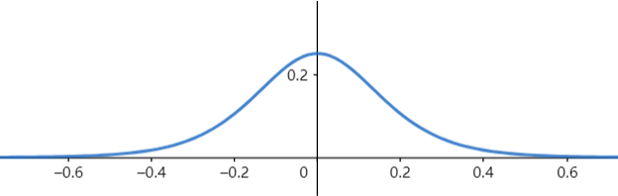
\includegraphics[width=0.6\textwidth]{undergraduate-thesis/images/neural-rgbd weighting function.png}
    \caption{公式\ref{eq: omninerf-basedline-weighting}所计算的权重函数分布。}
    \label{fig:omninerf-baseline-weighting}
\end{figure}

通过公式可以看出,距离函数较小的值将被赋予更大的体渲染权重。当距离函数通过这一函数映射到点权重后,我们可以将体积渲染公式改写为:
\begin{equation}
    \hat{C}(r) = \frac 1 {\sum_{i=0}^{N-1}w_i}\sum_{i=0}^{N-1}w_i\cdot c_i
\end{equation}

\begin{figure}[t]
    \centering
    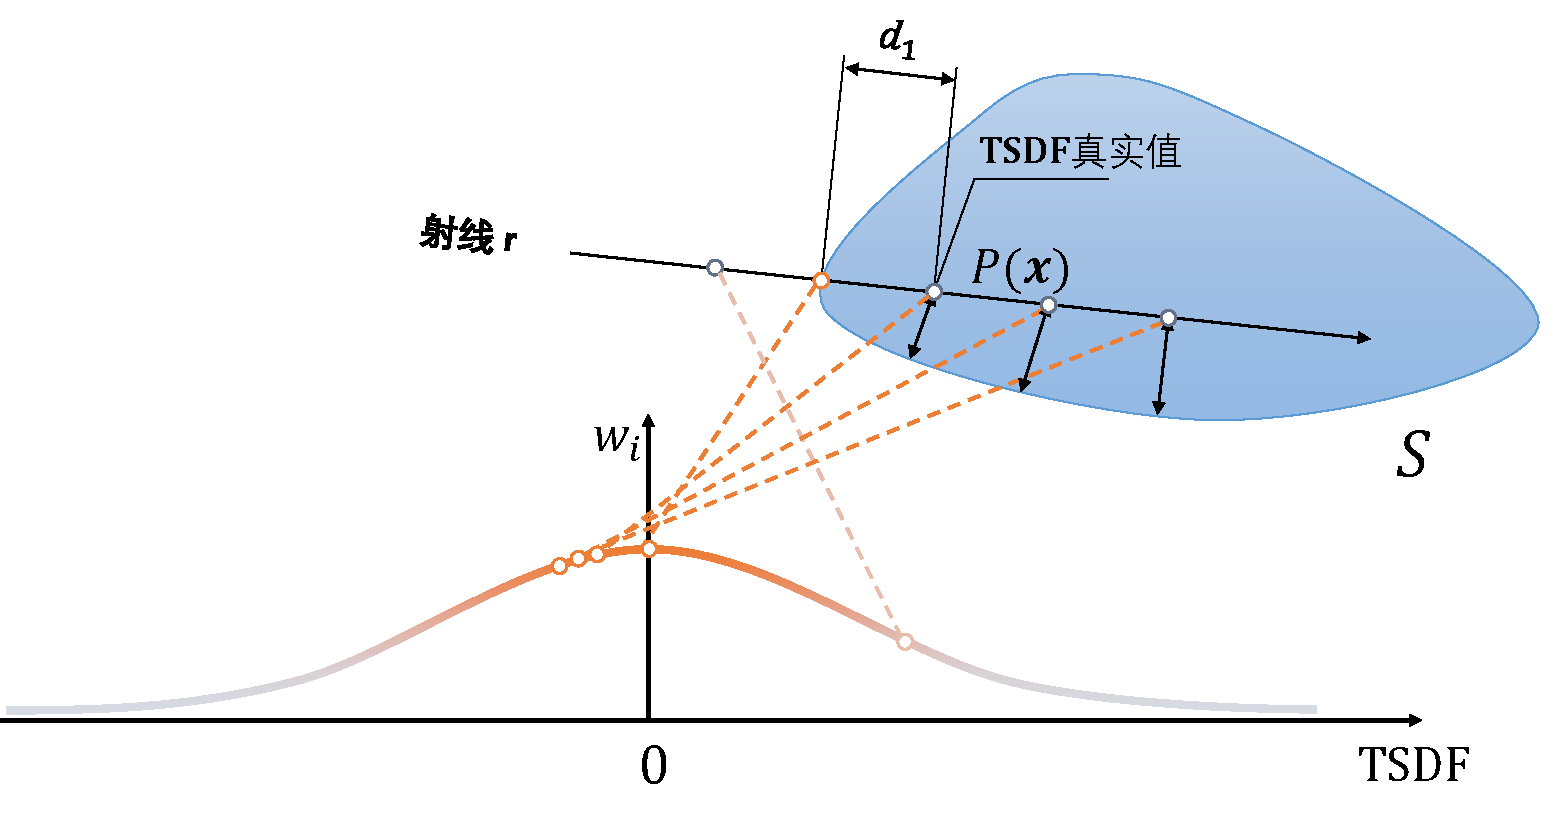
\includegraphics[width=\textwidth]{undergraduate-thesis/images/omninerf-error2.pdf}
    \caption{混合隐式场内在误差的二维示意图}
    \label{fig:omninerf-internal error}
\end{figure}

在这样的框架下, 我们描述一种由混合隐式场方案引起的系统误差。对于隐式表面$\mathcal{S}$,假设我们发射的光线$\mathbf{r}(t)$与表面$\mathcal{S}$在$t=t_0,t_1$处分布相交($t_n<t_0<t_1<t_f$),且光线$\mathbf{r}(t)$在表面$\mathcal{S}$几乎相切处入射(如图\ref{fig:omninerf-internal error}所示)。

对于$t\in[t_0, t_1]$区间中的采样点$P(t_{k_1}), \dots, (t_{k_N})$,这些点由于均位于表面$\mathcal{S}$内部,因而在体积渲染过程中,应占有较小的权重。然而,由于光线沿表面入射,当表面较为光滑时,有:
\begin{equation}
    0\approx w(t_{k_i} - t_0) << w(f_{SDF}(t_{k_i})) \approx w(0),
\end{equation}
其中$w(t_{k_i} - t_0)$较好地反映了点$t_{k_i}$处的体积,而实际预测值$w(f_{SDF}(t_{k_i}))$远远大于该点的真实密度。

由于点$t_{k_i}$靠近曲面$\mathcal{S}$表面,因而在辐射场中,该点求得的辐射颜色接近于其最近表面点$p_{k_i} + \nabla f_{TSDF}(t_{k_i})\cdot f_{TSDF}(t_{k_i})$的颜色。从而在体渲染过程中产生颜色混淆的效果。
\begin{equation}
    \hat{c}(p_{k_i})\approx\hat{c}\left(p_{k_i} + \nabla f_{TSDF}(t_{k_i})\cdot f_{TSDF}(t_{k_i})\right)
\end{equation}


\section{结合深度输入的混合隐式场距离-深度二义性}
除了前文提到的使用混合隐式场作为场景表示时出现的隐式场内在误差,我们在本节中还将介绍使用深度信号作为混合隐式场监督信号时出现的距离-深度二义性。在第二章,我们介绍了现有方法\cite{azinovic_neural_2022}在使用深度监督信号时在截断区域内所使用的深度损失函数:
\begin{equation}
    \mathcal{L}_{tr} = \sum_{p_{tr}}(f_{TSDF}(p_{tr})+t_{tr}-D)^2,
\end{equation}

该损失函数用$\hat{f}_{TSDF}(p_i) = D(\mathbf{r})-t_i$估计$p_i (p_i \in \mathbf{r})$点的截断符号距离函数。如图\ref{fig:omni-nerf depth error}所示,这个估计会对隐式场准确几何内容的学习产生很大的影响:当我们分别从两个视角$\mathbf{r}_1, \mathbf{r}_2$观察到同一空间点$P$时,由于该点到观察视角起点距离不同,由上述过程估计所得的对同一点的截断符号距离函数值$d_1, d_2$也不同,则当使用这两个不同的估计值同时作为点$P$的截断距离函数真值进行反向传播时,网络不能学到任意一个真实的TSDF值,从而导致结果模糊、计算资源浪费的结果。

\begin{figure}[ht]
    \centering
    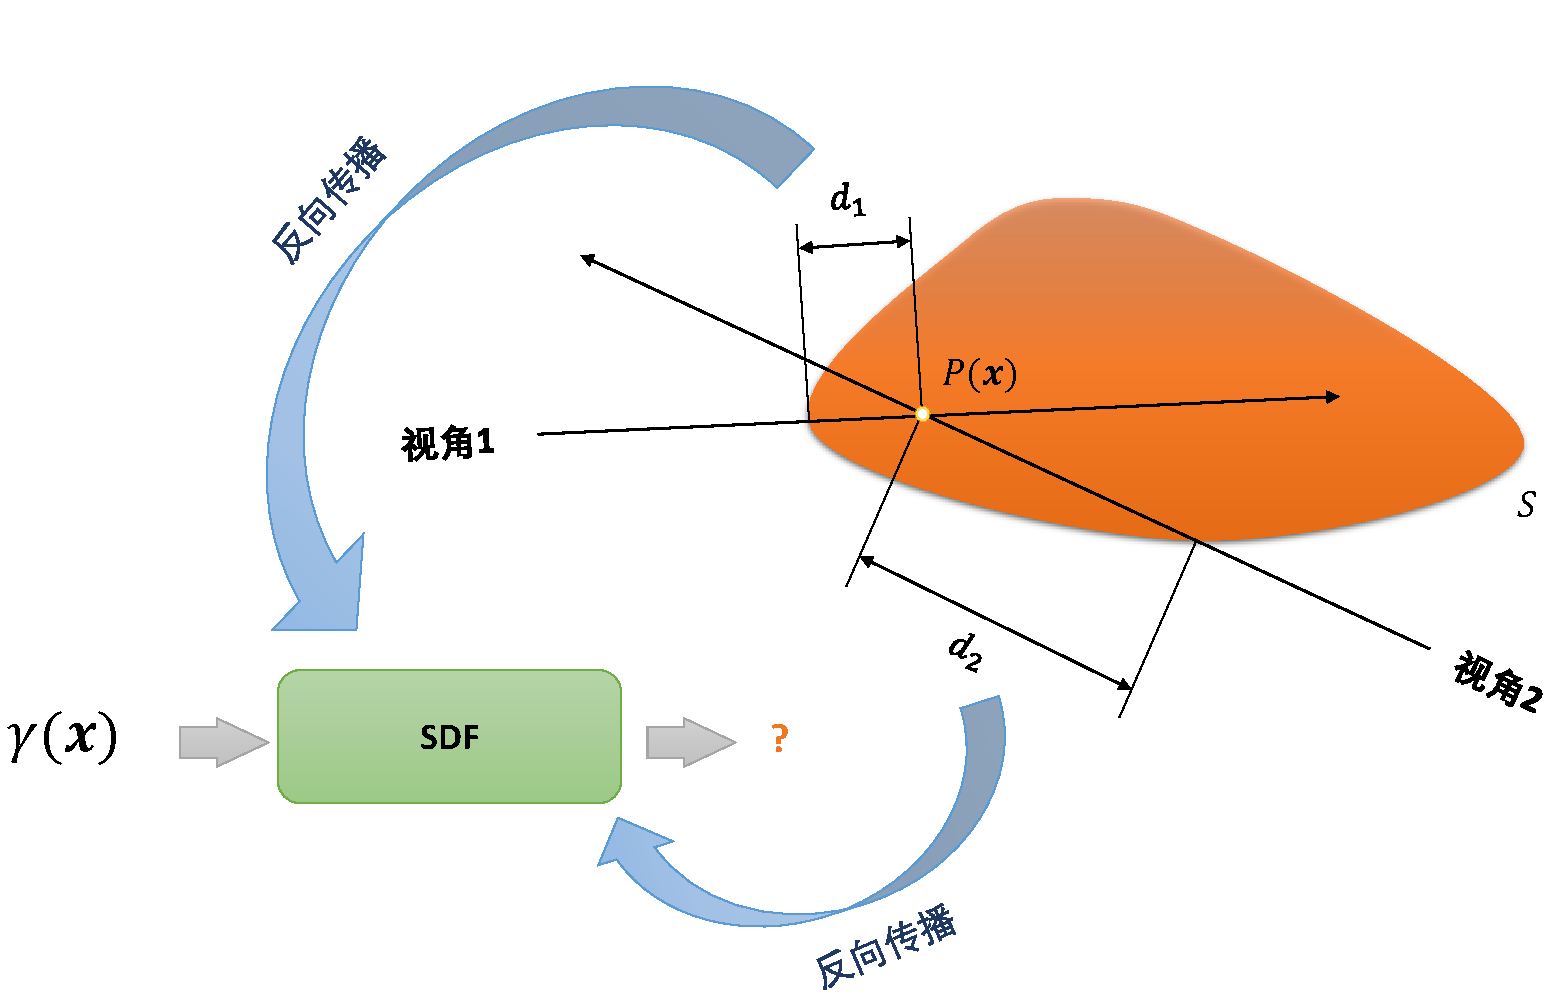
\includegraphics[width=\textwidth]{undergraduate-thesis/images/omninerf-error1.pdf}
    \caption{深度监督信号下的混合隐式场二义性示意图。}
    \label{fig:omni-nerf depth error}
\end{figure}


\section{基于全方向距离场的混合隐式场表征}
通过分析上面提到的两种误差,我们发现他们都是由于现有基于符号距离场的混合隐式表征技术方案在距离场设计上没有考虑到多视角的视角相关性,即应该使用随视角方向变化的距离函数计算权重。

基于这一观察, 在本课题中,我们提出基于全方向距离场的混合隐式表征方案。全方向距离场(Omnidirectional Distance Field, ODF)接受位置和方向的五维输入数据$(x,y,z,\theta,\phi)$,输出视角相关的距离函数值。全方向距离函数值代表了空间点$\mathbf{x}=(x,y,z)$在方向$\mathbf{d}=(\theta,\phi)$上最近表面的无符号距离。
\begin{equation}
    f_{ODF}: (\mathbf{x},\mathbf{d})\to \mathbb{R}_+
    \label{eq: omninerf-odf function}
\end{equation}

注意到全方向距离函数可以分解为符号距离场和一个全方向距离残差函数的和:
\begin{equation}
    f_{ODF}(\mathbf{x}, \mathbf{d}) = |f_{SDF}(\mathbf{x})| + f_\Delta(\mathbf{x}, \mathbf{d})
    \label{eq: omninerf-odf decomposition}
\end{equation}

我们设计了如图\ref{fig:omninerf-model}所示的网络。输入$\mathbf{x}$首先通过符号距离场得到$\mathbf{x}$的符号距离,通过将网络输出的几何参数继续前传,同时输入观察方向$\mathbf{d}$,计算空间点的全方向距离残差函数值$f_\Delta(\mathbf{x},\mathbf{d})$和辐射颜色$\mathbf{c}_i$。

\begin{figure}[ht]
    \centering
    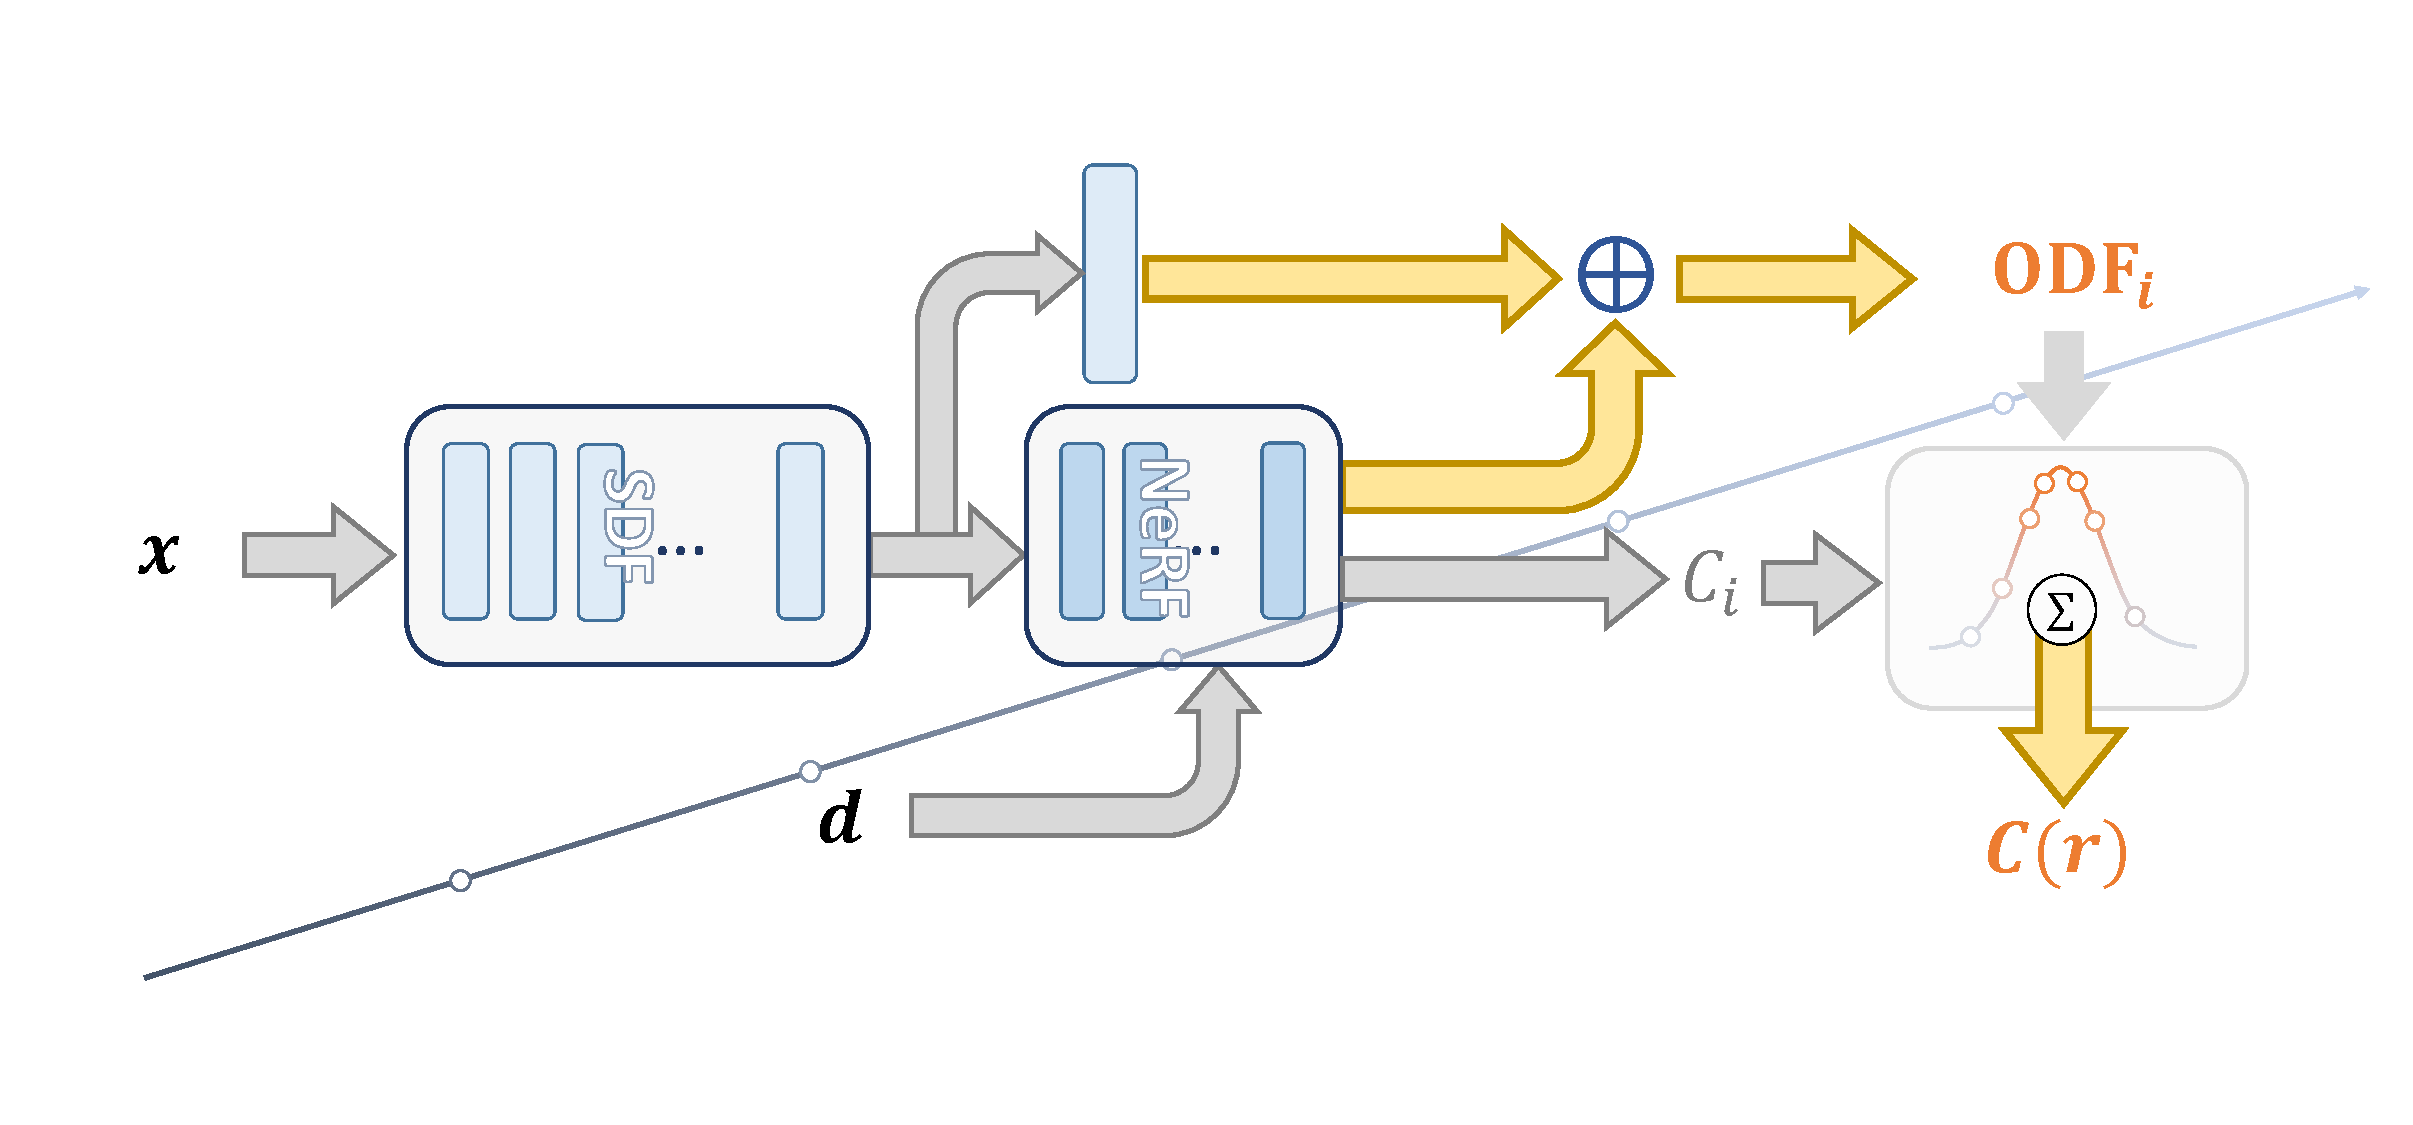
\includegraphics[width=\textwidth]{undergraduate-thesis/images/omninerf-model.pdf}
    \caption{基于全方向距离场的混合隐式表征方案}
    \label{fig:omninerf-model}
\end{figure}

通过将符号距离函数和残差函数重新组合,我们便可以得到全方向距离函数值,将该值按照现有体积渲染方案经过积分,便可以在一条射线上得到渲染颜色$C(\mathbf{r})$。 可以验证,我们提出的混合隐式场融合方案可以从理论上解决混合隐式场的内在误差和深度监督后的距离-深度二义性。

\section{场景表示实现}
在前面几节中,我们基于两种现有方法中观察到的误差和二义性,在理论上提出了可以去除这两种误差的解决方案,在本节中,我们详细描述使用全方向距离-辐射混合隐式场的实现方案。

我们在第\ref{chapter:related-work}章中介绍了现有的主流场景表示方法,其中,基于哈希体素网格的场景表示可以准确地建模场景细节但需要占据较大的存储空间,而基于多平面的张量分解场景表示在准确性上有所下降,但可以用更低的存储空间达到相媲美的效果。在本课题中,我们结合这两种不同的场景表示,使用一个较低分辨率的哈希体素网格建模场景细节,并使用一个更高分辨率的多平面作为辅助,以达到高效的准确场景地图骨干模型。我们的网络结构图如图\ref{fig:omninerf-scene-representation}所示。

\begin{figure}[ht]
    \centering
    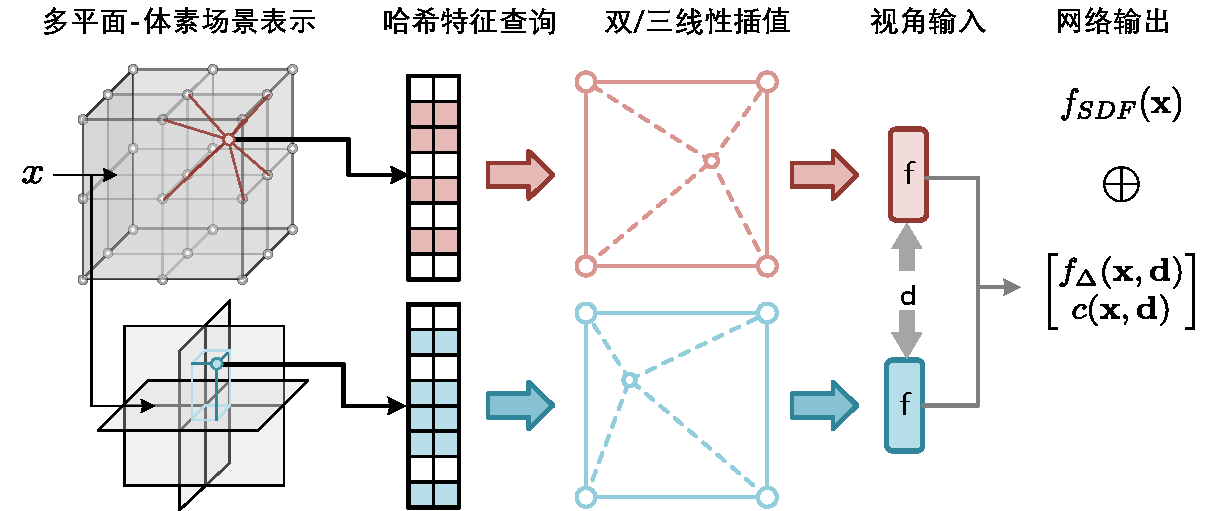
\includegraphics[width=\textwidth]{undergraduate-thesis/images/omninerf-scene-representation.pdf}
    \caption{场景表示模型架构图}
    \label{fig:omninerf-scene-representation}
\end{figure}

\subsection{优化全方向距离-辐射隐式场}

\section{本章小结}